\chapter{Creating a Proof of Concept Use for ScienceIE data}
\section{Concept and Specification}
Having completed systems to handle the information extraction, the next major part of the project was to explore how this information can be utilised for researchers. 

The most obvious domain for using summary information about a set of resources is search. Being able to efficiently search through a large set of documents to quickly find more useful information is a very useful thing. The focus of this section is to explore using the key phrase information in an efficient and convenient way to aid in user query across the ScienceIE data set. 

The ScienceIE data set is specifically being used because that is what the algorithms in this project are designed for. The problem of handling longer, full publications has been discussed, so to not complicate this investigation further, the standard short documents of ScienceIE shall form the database of documents.

The following requirements are presented for the POC system to conform to are:
\begin{enumerate}
	\item As a basis to make the system usable, the ability to list papers in the database, and the ability to present all the information about a paper on one screen. The ability to download the extractions in the BRAT format should also be made available. 
	\item A search system for the key phrase information gained. This should allow the input of a user query (plain natural language text), with an option to give some indication of the classification of the information they are interested in (i.e. \textit{task}, \textit{process} or \textit{material}).
	\item The ability to add papers dynamically to the database throughout run time. This means not only should the system support the creation of new paper records, but also the automatic processing of that paper through all 3 subtasks of ScienceIE, with the results being available to the search system.
	\item Some way of conveying summary information about the extractions contained in the system. While not essential for search, having a convenient way for the developer and users to take a snapshot of what is contained in the system is useful for evaluation purposes, including giving an indication of how many papers are included and their processing status.
\end{enumerate}

\section{Background and Technology Review}
\subsubsection*{Existing Search}
Two popular, publicly available search engines have been examined to extra some well designed features from. These are Google Scholar\footnote{\href{https://scholar.google.com/}{https://scholar.google.com/}} and ScienceDirect\footnote{\href{https://www.sciencedirect.com/}{https://www.sciencedirect.com/}}, and appendix \ref{appendix:searcheg} shows screen shots of both web sites given the same query. Common features are:
\begin{itemize}
	\item Limited results per page (10 on Google Scholar, 25 on ScienceDirect),
	\item The total number of documents selected and the time it took to do this is displayed to the user,
	\item Filtering options, including by date,
	\item The title of a result is followed by a snippet of the document, with relevant words highlighted in some way,
	\item The title is a link to an individual results page which presents information about the document, but there are also links to directly get the document downloaded.
\end{itemize}

\noindent Some custom features on each website are:
\begin{itemize}
	\item ScienceDirect supports searches with multiple parameters, including query fields specifically for author, title, pages, etc...
	\item ScienceDirect also supports custom numbers of search results per page; 25 is the default, but the user can receive 50 or 100 results per page if they wish,
	\item Google Scholar present \textit{related searches} to allow the user to navigate sideways towards their target paper, rather than straight down to it,
	\item ScienceDirect features a \textit{recommended} section at the top where it showcases several publications it believes to be the most relevant.
\end{itemize}

Given the data set available in this project, most of these ideas presented by Google Scholar and ScienceDirect can be implemented. However, as ScienceIE's data is purely text snippets of documents, author, real title, publish information and more are unavailable, meaning any system created here cannot support filtering by these features, or display that information. An original hope of the developer was to include a more advanced search, potentially including a PageRank type system \cite{Page1998} where the links would be based on referencing, but unfortunately without even the reference information for each paper available, this is impossible to achieve whit the ScienceIE dataset.

The search on these two websites is likely be based on latent semantic analysis (\cite{Landauer1998} and \cite{AswaniKumar2012}) which looks at the similarities between search terms and attempts to take into account context. This method of representing words in a vector space prepared for querying is a popular method of document retrieval. This method of querying could potentially be modified to involved more weighting of tokens if the are included in key phrases, or be used to inspire a new algorithm that uses key phrase information to help with weighting word importance.

\subsubsection*{Available Technologies}
The goal with this project is to prove a use of the data produced as part of ScienceIE through some application. To make this application available for use, a web based service will be created that allows any user to join without the need for complex setup. The benefits of this include not having to distribute installation media and update media, along with centralised management of any database of information and being able to immediately make available new features.

In terms of storing information, popular database technologies were surveyed. The stack overflow survey 2017 listed MySQL\footnote{\href{https://www.mysql.com/}{https://www.mysql.com/}} as the most used SQL platform by developers on the sight\footnote{\href{https://insights.stackoverflow.com/survey/2017\#technology-databases}{https://insights.stackoverflow.com/survey/2017\#technology-databases}}. One reason for this is that some competitive SQL platforms require licensing (especially when commercial use is considered), such as Oracle SQL, while MySQL is open source and can be used more freely. The platform can be easily acquired and installed on various platforms (with major Windows and Linux operating systems supported), with largely straight forward initial configuration (for a project of this scale). The standard MySQL installation also includes the MySQL Workbench, which includes a convenient tool for building a relational database schema\footnote{\href{https://dev.mysql.com/doc/workbench/en/wb-data-modeling.html}{https://dev.mysql.com/doc/workbench/en/wb-data-modeling.html}}, with the ability to export SQL scripts to build the designed database in a single execution (including tables, relations and users with certain access rights). 

One of the most popular Java web frameworks available is Spring. Spring provides functionality to route requests to certain Java classes for processing, including the passing of any parameters with some degree of automatic validation, and the ability to process Java Servlet Pages (JSPs) which are compiled at run time to delivery varying pieces of information to the end users. It supports the standard \textit{model-view-controller} (MVC) design pattern. To keep the focus on the use of data processed in this project, a convenient web container is desired, and that is what Spring Boot\footnote{\href{https://projects.spring.io/spring-boot/}{https://projects.spring.io/spring-boot/}} provides. This packages the Spring technology stack, web server technology (for example, Apache Tomcat) and any extra libraries required into a single, executable, Java project, making heavy use of annotations for the minimal configuration required. This makes it an extremely portable and (in terms of environment and system configuration) light weight application to set-up and run, which reflects as part of their projects mission statement to get developers "up and running as quickly as possible". It is a young project, with the original version being released in 2014 and version 2.0 being released during the course of this project, meaning it is built to work with the current standard of industrial Java technologies - so while this project is aiming to build a simple application, it shall have some powerful technologies standing behind it.

One of these technologies is Hibernate\footnote{\href{http://hibernate.org/}{http://hibernate.org/}}. This integrates with the Java Persistance API (JPA), supported by Spring, for extremely simply database interactions with many functions being supported by default. It combines a simple Java object which holds fields relating to each of the column in a database entity (table), and an abstract \texttt{CrudRepository} class which can be extended from to make a data access object which can retrieve records from a database and update them as well. Methods can be added to the extended class to make more complex queries, and either plain English can be used in the method name to define the query, or the specific SQL query statement can be specified if required\footnote{A guide to using this technology is freely available on Spring's website and is presented in a very simple manor. It can be viewed at \href{https://spring.io/guides/gs/accessing-data-jpa/}{https://spring.io/guides/gs/accessing-data-jpa/}} Furthermore, when fields are foreign keys of other entities, rather than being of an \textit{ID} type such as \texttt{Integer} or \texttt{Long}, the class representation of the foreign entity can be used instead, and Hibernate will automatically populate it with the correct object.

\section{Core Component Design}

\subsection*{Design of the Services}
There are four key requirements of the POC system which cover a large amount of usability. The first requirement is very simple. Two pages are required for this:
\begin{itemize}
	\item The first is simply a list of papers, each selectable. When selected, the user will be taken to the next paper described.
	\item The second page, for displaying information about a paper, should begin with the title at the top, a section in the middle for the original text, and finish with a list of key phrases and relations. The key phrases, as a minimum, should be annotated on the main text as well.
\end{itemize}

The second requirement is covering the question of search. A new algorithm is proposed that includes the key phrase information about a paper. Using the concept of combining the TF-IDF scores of both the tokens from documents as well as from in the query to try to prioritise papers is utilised with a scaling factor, defined by the presence of key words in a paper. When searching, the following process should happen:
\begin{enumerate}
	\item The query string shall be tokenized, and every token shall have its TF-IDF score calculated (relative to the training set, as all TF-IDF scores are calculated).
	\item A set of papers are selected, with the criteria of needing to have at least one of the tokens from the query as a substring of the entire text.
	\item For every paper selected, the tokens that relate to the search query are extracted. The extracted token may not be the same as the query token, as the query token could be a substring of the extracted token.
	\item For every paper, for every unique token extracted in the previous step, the TF-IDF value of the extracted token is multiplied by the TF-IDF value of the query token it relates too as a \textit{TF-IDF weighting}. 
	\item For every paper, for every token extracted, a \textit{scaling factor} is then calculated. Beginning at one, it is incremented by one for every key phrase (for the given paper) a query token appears in.
	\begin{itemize}
		\item If a user is \textit{focussing} on a certain classification of information (e.g. \textit{task}), then only the specified types of key phrases are used when scaling.
	\end{itemize}
	\item The \textit{TF-IDF weighting} for each token extracted from a paper is then multiplied by the \textit{scaling factor} calculated for the token.
	\item These multiplied values are then summed for each paper. The sum is the papers score.
	\item The papers are ordered by score, with the largest score being first to be presented to the user, and the lowest last.
\end{enumerate}

This should, as a base line, retrieve all relevant papers to a users query with a reasonable ordering relative to the TF-IDF values of the query words. Furthermore, it should prioritise terms that are part of key phrase of documents, which should list documents specifically addressing certain concepts higher than documents mentioning them, which is an ideal use for the key phrase information extracted. A problem which may occur is when a search term with a high TF-IDF value is found (as it has a low occurrence in the document it appears in) and a low TF-IDF word which happens to appear in key phrases. As the multiplier may be large for the low TF-IDF valued word, it may overtake the other, more important word in overall paper score, which may not be idea for the user. However, this isn't expected to happen often, as low TF-IDF valued words are unlikely to be part of key phrases, as (implied by their TF-IDF score) they are not critical pieces of information in the document. 

The next requirement is the ability to add new papers. In terms of user input, this is fairly simple, as a string will be taken in and can be treated as a file descriptor. Given many other jobs need completing in this project, and a web resources paper type wasn't created in the NLP system, to for fill this requirement, any paper location added shall be treated as a file URI and looked for on the host system's disk. This can then be loaded into the system and processed through each of the subtask systems.

To complete the processing, a paper will need a status associated with it. This status should describe what the next stage processing the paper should experience is. In order, the processes are: \textit{preprocessing}, \textit{key phrase extraction}, \textit{key phrase classification}, and \textit{relation extraction}. To complete the subtasks, the solutions with the best found configurations in the NLP system shall be used. The use of the set of SVMs this will require can be optimised: rather than training for every paper, the first time a SVM is used it can be trained, then serialised and saved to disk. Every time after that, it can be loaded back into memory without the need for hours or retraining. Furthermore, given the SVMs and Word2Vec take up a large amount of memory, rather than processing one paper at a tie end-to-end, all papers needing an action being completed can be processed at once with its required resources being loaded and reused throughout, before unloading ready for the next stage of processing which will work on all papers in that status as well.

Overall, this should all the efficient processing of all papers in the system. As the extracted content is predicted, it can be immediately added to the database allowing the search and other systems to immediately update with the latest information.

Finally, the last requirement is a little open to interpretation, as all that is required is the display of some summary information about what is in the database. Two data visualisations are proposed:
\begin{itemize}
	\item The first is a simple pie chart. It shall have three segments, each representing the percentage of key phrases that are each classification. Next to the pie chart (aside from a legend or similar describing each segment) the number of key phrases should also be displayed, so the number of each classification can be understood.
	\item The second is a larger visualisation. Three word clouds should be created, made up of the tokens of key phrases extracted, one for each classification. To determine the size of a token in a word cloud, two values are proposed: the words commonality (i.e. each words occurrence is counted), and it's TF-IDF value should be used. While both shall be tested, it is expected using TF-IDF will produce more interesting results, as this will allow words with high importance to stand out over words which are still key phrases, but less important. This should give a user an insight into what information is in the system, and ideas for what to search for to achieve better results given they know what words are in the key phrases, rather than highlighting the potentially less interesting words.
\end{itemize}

\subsection*{Database Design and Entity Relationship Diagram}

\begin{figure}
	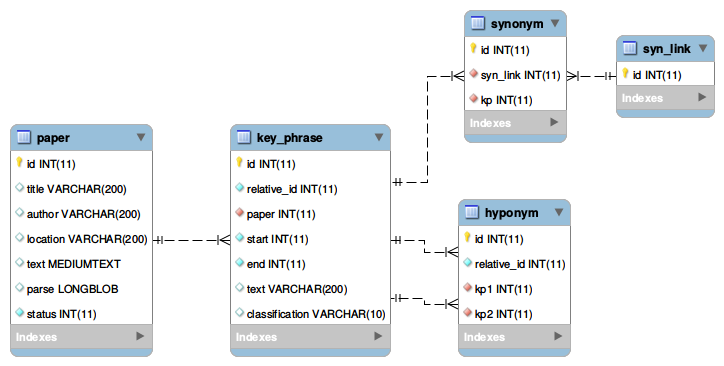
\includegraphics[width=\textwidth]{img/fypdberd.png}
	\caption[Database Entity Relationship Diagram]{The entity relationship diagram that supports this proof-of-concept system, as exported from the MySQL Workbench tool kit. Primary keys are represented by gold keys, foreign keys are red diamonds, normal fields are blue diamonds and hollow blue diamonds indicate the field is nullable. Types for all fields in all entities are also shown. The Java representation of these entities share the same name in all cases, converted to camel case, aside from the entity titles which have \texttt{DAO} appended (standing for \textit{data access object}) as without this the class names would clash with those used in the NLP system, which would have been confusing to program with. As examples, the \texttt{paper} entity was \texttt{PaperDAO} in the Java project, but an \texttt{id} field would remain \texttt{id} in the Java code to follow the standard.}
	\label{figure:dberd}
\end{figure}

The support storage and query of the data produced by the ScienceIE task, a suitable database must be designed and created. Given a lot of the required entities had been created as part of the NLP system, the data base design heavily inherits the classes and fields from this. The full design for the database is shown in figure \ref{figure:dberd}

The \texttt{paper} and \texttt{key\_phrase} entities are largely the same as their equivalents in the NLP system. Of course, rather than having a list of key phrases held within the \texttt{paper} entity, the \texttt{key\_phrase} entity has a field to store a reference to its parent \texttt{paper}. The \texttt{paper} entity also has two fields no in the NLP system: a \texttt{status} which was discussed above, and a \texttt{parse} which holds a serialised \texttt{Paper} Java object. This allows the preprocessing to take place and for that information to be stored directly in the database with its parent record, removing the need for re-computation of preprocessing every time the paper is called from the database.

The method for storing hyponyms and synonyms is slightly different to the NLP system. Rather than being part of a relations list the parent paper record holds, instead each relation holds the \texttt{key\_phrase} references they are a relation of. The original \texttt{paper} can still be retrieved through retrieving the referenced \texttt{key\_phrase} records. The \texttt{hyponym} record holds the two \texttt{key\_phrase} records it is a relation of, as well as a relative ID, which is the ID of the hyponym relation relative to the individual paper it is from. The \texttt{synonym} relation is a little more complex. While the NLP system created didn't support more than two way synonym relation extraction and there was only one example of a three way synonym relation in the ScienceIE data set, to support the range of relations defined as part of ScienceIE these synonym entity has to support one synonym referencing a variable amount of \texttt{key\_phrase} records. Therefore, to avoid a many-to-many relation between entities, each \texttt{synonym} record holds a reference to a \texttt{syn\_link}, the concept being a set of synonyms, each referencing one \texttt{key\_phrase}, all reference the same \texttt{syn\_link} record, which makes the synonym relation between the set of referenced key phrases. Having \texttt{syn\_link} also provides a convenient way to count he number of synonyms in the system.

\section{Implementation}
This section shall cover the infrastructure of the POC system and how the requirements are handled. The graphical user interface (GUI) information shall be described later in the \textit{Web Interface} section.

\subsection*{Project Configuration}
The creation of the project involved including various dependencies in the \texttt{pom.xml} file and setting up the launch configuration for Spring Boot.

To include Spring Boot, \texttt{pom.xml} was configured as described on the Spring Boot website, along with a connector package for MySQL\footnote{\href{https://spring.io/guides/gs/accessing-data-mysql/}{https://spring.io/guides/gs/accessing-data-mysql/}}. 

\begin{figure}
	\begin{lstlisting}[language=XML]
<dependency>
  <groupId>xyz.tomclarke.fyp</groupId>
  <artifactId>fyp-nlp</artifactId>
  <version>0.0.1-SNAPSHOT</version>
  <!-- Stop logging dependency errors -->
  <exclusions>
    <exclusion>
      <groupId>ch.qos.logback</groupId>
      <artifactId>logback-core</artifactId>
    </exclusion>
    <exclusion>
      <groupId>org.slf4j</groupId>
      <artifactId>slf4j-log4j12</artifactId>
    </exclusion>
  </exclusions>
</dependency>
	\end{lstlisting}
	\caption[Configuration to set the NLP system as a dependency in Maven]{The Maven configuration for listing the NLP project as a dependency, as used in the POC system. Note, the exclusion (as discussed) are to remove logging dependency conflicts using Spring Boot causes; this may break logging if another system uses this configuration but doesn't have its own logger available.}
	\label{figure:nlpdependency}
\end{figure}

To use the NLP system built in this project, Maven also needed to be told to import this so it can be used to generate information about given papers when the full system has been developed. Given the NLP system has been compiled and installed to the local Maven repository (as it is not hosted anywhere), the configuration shown in figure \ref{figure:nlpdependency} will include the NLP system in a compiled project. Doing this also sets any dependencies of the NLP system as dependencies of this system, so they do not need to be re-listed as dependencies. The unfortunate effect of this is where there are conflicts between dependencies, which is what happened in this project. The logging included in Spring Boot was an alternate version to that in the NLP project, and while it didn't damage any part of the system, on every boot it would choose one of the loggers and print out many error messages warning the developer against it. Therefore, the conflicting dependencies in the NLP system were excluded to remove this problem, and this was done to the NLP system rather than to Spring Boot as this problem may occur if the NLP system was used in another project including other dependencies, so it made sense to list how to fix it for the NLP system dependency. 

For the system to launch, some basic configuration had to be set. There is an \texttt{application.properties} file in the Java resources with the following parameters (with explanations as to why those were chosen appended):
\begin{itemize}
	\item \texttt{server.port=8080} 8080 is a standard port for testing web applications on. Furthermore, port 80 needs administrative privileges to be used ever time the application is launched, which would not only be frustrating to a developer, but not supporting good security standards if there was a vulnerability in the web service. The router the developer system was sitting behind, through port forwarding, allowed incoming connections on port 80 to be directed to 8080 on the developer system, so when connecting via web browser, no port would be needed to be specified.
	\item \texttt{debug=false} If \texttt{true} was set, this would output all debug information to the console. Given the log4j configuration being used output all debug information to disk, there was no need to have it also in console, making it harder to see what was going on while running.
	\item \texttt{spring.jpa.hibernate.ddl-auto=none} This parameter has several different possible values. \texttt{none} means the connection to the database is standard, allowing the Java application to commit reads and writes. Other values were possible, which would support (if the database hasn't been setup) automatic configuration of the database based on the entity declarations. While this could have been useful, control of configuring the database being left to the entity relationship software included in the MySQL workbench seemed preferable.
	\item \texttt{spring.datasource.url=\newline jdbc:mysql://tomclarke.xyz:3306/fyp?verifyServerCertificate=false\&useSSL=true} This is the JDBC connection string, allowing the system to find and connect to the database. To increase security, encryption of the connection through Secure Sockets Layer (SSL) is enabled, but as the database server is not configured with any certificate, this is set to be ignored.
	\item \texttt{spring.datasource.username=fyp\_user} This is simply the database user setup for the system to use. The permissions on this user were restricted to read and write of data in the \texttt{fyp} database, so if the application is compromised the database connection can't be used to read information from other databases on the same instance, or change the configuration of the database system. 
	\item \texttt{spring.datasource.password=$<$password$>$} This is the password of the database user for the system to login with.
\end{itemize}

Several parts of the above are concerned with, as well as required configuration, security of the database and system as whole, and while this project is not concerned with security, it is seen as good practise to include these features.

Finally, the class \texttt{FypGuiApplication} needed to be created, as it is this class that contains the classic \texttt{public static void main(String[] args)} method that starts the whole program. Along side the opportunity to include any other pieces of configuration completed through Java code, this initiated the Spring MVC technology stack.

\subsection*{Implementing The Requirements}
To complete the requirements, several internal services needed to be created. For the simple display of data (for the first requirement), simple database queries could be ran and the data immediately propagated to screen. However, the other requirements require more complex solutions. 

Before continuing, the following classes are all annotated with \texttt{@Service}. This tells Spring to instantiate these classes (each one as a singleton) and allows them to be automatically injected into other objects. For example, \texttt{PaperUtil} is a class which provides utility methods for the system (including holding training paper information and utilities for calculating TF-IDF values and for loading serialised papers). It has a \texttt{@Service} tag, and if another class wishes to use it, \texttt{@Autowired private PaperUtil util;} can be added as a field in the class and Spring will automatically make the instantiated \texttt{PaperUtil} object available.

To handle search, two classes were created. \texttt{PaperSearch} handles the incoming \texttt{SearchQuery} object, which is all the information about a users query. Using this information, \texttt{PaperSearch} retrieves all the database information required to complete the suggested algorithm for calculating paper scores. Each paper, one by one, is then passed to \texttt{PaperScoreCalculator.calculatePaperScore} to have its score calculated. The reason for a second class being used here is it allows the user of asynchronous technology. The method called is annotated with \texttt{@Async}, and returns \texttt{CompletableFuture$<$Double$>$} (score is measured in the \texttt{Double} data type), which causes the processing calling the method to not wait for a return value and carry on, effectively making a new thread every time the method is called. The effect this has is that a loop can be made, calling this method for every paper, which immediately returns a list of \texttt{CompletableFuture$<$Double$>$}. This list, effectively made up of a set of threads, can be joined on later, meaning execution will only continue past the \textit{join} once all threads have finished their calculations. The configuration for this pool of threads is completed in the \texttt{FypGuiApplication} class which starts the system. Given the test set, the data set that will be input to the system, is 100 items large, the thread pool was given a size of 100, so if a query covering all papers was requested the entire query could be parallelised. This should allow fast execution of this case, and should also cope with several users doing multiple queries simultaneously without much slow down. From testing, using this asynchronous method oppose to sequentially calculating a score for each paper saw some massive speed increases, which can be seen in table \ref{table:searchtimesasync}. Once the search is complete and the results ordered, the papers are converted to a \texttt{SearchResult} model which contains the key information for the user to see while searching.

\begin{table}
	\centering
	\begin{tabular}{ C{4.5cm} | C{4.5cm} | C{4.5cm} }
		\textbf{Query} & \textbf{Time in seconds (sequential)} & \textbf{Time in seconds (asynchronous)} \\
		\hline
		a & 80 & 23 \\
		the & 10 & 3.8 \\
		support vector machine & 0.5 & 0.2 \\
	\end{tabular}
	\caption[Search Times with and without parallel execution]{Times for searches to complete, before and after asynchronous calculation of paper scores were added.}
	\label{table:searchtimesasync}
\end{table}

The next requirement to implement was the input and processing of all papers. Upon input of a new paper by a user, a new \text{paper} record was made. It simply held the location given of the paper and a status of 0. To pick up this new paper, the \texttt{PaperProcessor} class has a method \textit{processWaitingPapers}. This method is annotated with \texttt{@Scheduled(fixedDelay = 60000)}, which tells Spring to run this method once every 60000 seconds (60 minutes), which is a long time but stops it regularly doing requests to the database making that connection busy, to a database that should rarely have new papers added given web resources are not supported. This method searches for all papers with a given status, one status at a time (starting at 0 and ending at 3). This covers all \textit{in progress} papers. It then applies a \textit{task} to it, which is the processing step from the NLP system. In this sense, it makes maintenance of this system fairly simple, as if there was a need to test another process for a subtask, the class using this process could be listed and \texttt{PaperProcess} would apply it automatically. If there was any issue with processing a paper, its status would be set to -1 so it would not be processed again, and would be easy to find as an error paper in the database.

Each \textit{task} was implemented in a class which implemented the \texttt{NlpProcessor} interface. The classes created were, in order of processing, \texttt{PreProcessor}, \texttt{KpSvm}, \texttt{ClassW2V} and \texttt{RelSvm}. The interface defined three required methods which \texttt{PaperProcess} runs in order: \texttt{loadObjects()} which loads the required resources for that process to be run, \texttt{processPaper(Paper)} which is run on every paper to extract the required information using the components from the NLP system, and finally \texttt{unload()} which ensured the memory is cleared to allow for other classes to load in their required resources.

% TODO does the above make sense and cover everything...?

Finally, the information for the data visualisations needed to be prepared. The pie chart, listing the proportions of each classification of key phrase, were deemed simple to compute at run time, as it requires querying the database to find the count of each classification and simple division of that over the total number of key phrases. However, the key phrase word clouds need slightly more computation to display.

For each of the three word clouds, all of the key phrases for that classification need retrieving, tokenizing and their values (count or TF-IDF depending on the test) calculating. This takes some time, which is too long for a user to wait to view them, and will be the same for every query (unless the processing of papers is currently happening). Therefore, a cache was designed. This cache was built under the method \texttt{KeyPhraseCloudCache.updateCache()}, which has the special annotation \texttt{@PostConstruct}. This annotation tells Spring to run this method after the object has been created and any dependencies added through the \texttt{@AutoWired} made available, but before the web server is actually launched. This increases the system start up time, but means the word clouds are available to be send to an interface immediately. To ensure the clouds are up to date if papers are being processed, every time a set is processed under any task, this \texttt{.updateCache()} method is called again to regenerate the word clouds.

An important note on the architecture here is the use of TF-IDF, and that it requires a library of papers to be calculated. The training papers are loaded in the mentioned \texttt{PaperUtil} class, which also has a method with the \texttt{@PostConstruct} annotation which loads this information. These training papers can be retrieved by any other class (mainly for use in training the SVMs as part of the paper processing functionality), but are also used when a TF-IDF value is calculated. The potential problem if the word cloud builder tried to use \texttt{PaperUtil} to calculate TF-IDF before the training papers had been loaded in and prepared. However, as \texttt{PaperUtil} is a dependency of \texttt{KeyPhraseCloudCache}, Spring ensures the post construct method in \texttt{PaperUtil} is always ran before that of \texttt{KeyPhraseCloudCache} to ensure that any resources are fully loaded and ready to be used. 

\section{Web Interface}
\subsection*{Controller Infrastructure}
The web interface covers a series of different pages. Spring, supporting the MVC design pattern, allows for controller classes (annotated with \texttt{@Controller}) to load views in the form of JSPs, and pass them model information acquired from other services. In the case of forms where the user has to input some data, a model can be bound directly to the input fields on the page. When submitted, automatic validation (including type checking) can be done by Spring, and the controller can receive the model object for processing. Specified in the controller class, URIs are bound to specific controllers. The controllers can also have different methods for interpreting \texttt{GET} and \texttt{POST} requests, for which different parameters can be specified.

\begin{table}
	\centering
	\begin{tabular}{ C{3cm} | c | c | c | C{5.5cm} }
		\textbf{URI} & \textbf{Method} & \textbf{Controller} & \textbf{JSP} & \textbf{Functionality} \\
		\hline
		\texttt{/} & GET & \texttt{Home} & \texttt{home.jsp} & Return the title of the project and displays the pie chart visualisation. \\
		\hline
		\texttt{/add} & GET & \texttt{Add} & \texttt{add.jsp} & Returns the page to input a paper location on. \\
		\hline
		\texttt{/add} & POST & \texttt{Add} & \texttt{add.jsp} & Accepts a papers location, and if valid adds it to the database for processing. Returns a message indicating success or failure of the action. \\
		\hline
		\texttt{/search} & GET & \texttt{Search} & \texttt{search.jsp} & Returns the search input fields. \\
		\hline
		\texttt{/search} & POST & \texttt{Search} & \texttt{search.jsp} & On submission, validates the search and uses the \texttt{PaperSearch} service to do a search. It then returns the same page as before, with a table listing all results. Clicking on a row loads \text{/view} for that paper. \\
		\hline
		\texttt{/view} & GET & \texttt{View} & \texttt{view.jsp} & It accepts a paper ID as an input. It then loads the paper from the database (including all extraction information) and adds it to the JSP to be returned to the user. It shows the title, main text, and a table with all key phrases in. Relations were not shown due to no good way being decided upon to represent the information, but given the NLP system gives poor results for relations this features was not focussed on too heavily. \\
		\hline
		\texttt{/view/download} \texttt{/view/extractions} & GET & \texttt{View} & N/A & Given a valid paper ID as an input, this returns a stream of a text file containing the original document or the extractions in BRAT format, respectively. \\
		\hline
		\texttt{/kps} & GET & \texttt{KPView} & \texttt{kps.jsp} & Returns the shell of the page to display the word clouds on. \\
		\hline
		\texttt{/kps} & POST & \texttt{KPView} & N/A & Accepting a type parameter, it returns all world cloud information (tokens and TF-IDF values) in a JSON format. \\
		\hline
		\texttt{/kps/\{type\}} & GET & \texttt{KPView} & \texttt{kp.jsp} & Returns a page containing a table of all key phrases with a classification of the given \textit{\{type\}}. Each row is a link, and takes the user to the \text{/view} for its parents paper. \\
		\hline
		N/A & N/A & \texttt{Error} & \texttt{error.jsp} & This controller handles errors. The returned page includes the HTTP error code (for example 404: not found) and, if debug is enabled in \texttt{application.properties}, a stack trace of what went wrong. \\
	\end{tabular}
	\caption[Available Requests the POC Website Supports]{All available requests that are supported by the web site. The \textit{controller} is the name of the Java class that provides the functionality.}
	\label{table:webservices}
\end{table}

All supported URIs and request methods, with controller, JSP and function provided are listed in table \ref{table:webservices}. 

\begin{figure}
	\centering
	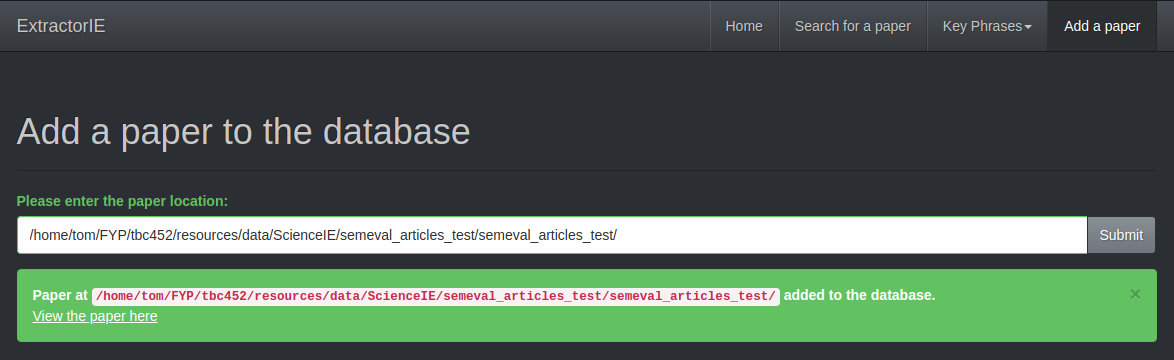
\includegraphics[width=12cm]{img/extractorie-add.png} \\
	\caption[The add of the website]{The add page of the website, with feedback to the sure shown giving indication of a successful paper addition to the system.}
	\label{figure:extractorieadd}
\end{figure}

When data is added to a JSP, it can often be directly printed out, however, some items are in lists (such as search results) which cannot be printed straight out. There are also cases where we wish to display one thing or another (for example, a success message or an error message) so there is the need to do \textit{if} statements in the JSP. The JavaServer Pages Standard Tag Library (JSTL) provides all the solutions needed here, as the \texttt{forEach} tag can be used to iterate down a list of data, and tags such as \texttt{if} and \texttt{choose} can be used to show or hide different parts of the page. The JSTL tags need to be imported on every page. An example of this, where it is used to give user feedback on the success of an action, is on the \texttt{/add} page, shown in figure \ref{figure:extractorieadd}

To ensure all pages have the necessary styling, scripts and navigation bar (which is essential for navigating through the website) are included on every page, the following tags are on every page:

\begin{lstlisting}[language=XML]
<jsp:include page="header.jsp"></jsp:include>
<jsp:include page="navbar.jsp">
  <jsp:param name="active" value="" />
</jsp:include>
\end{lstlisting}

\texttt{header.jsp} and \texttt{navbar.jsp} include all of the imports and generic styling every page should have applied.

\subsection*{Styling}
In terms of styling, to keep layout simple and text clear to read (as both of the example websites are), rather than building a consistent style from the ground up, Bootstrap\footnote{Bootstrap is made up of CSS files and JavaScript files, all of which are needed and can be retrieved from \href{https://getbootstrap.com/}{https://getbootstrap.com/}. At the time of development, version 3 was available.} was used. To give the website a slightly more unique feel, an on-line customer was utilised to help quickly develop an aesthetically pleasing and easy to read style\footnote{The \textit{slate} theme was used as a basis on \href{https://www.bootstrap-live-customizer.com/}{https://www.bootstrap-live-customizer.com/}.}.

To support Bootstrap and custom scripting in the web pages produced, jQuery\footnote{\href{https://jquery.com/}{https://jquery.com/}} was also included in the project.

\begin{figure}
	\centering
	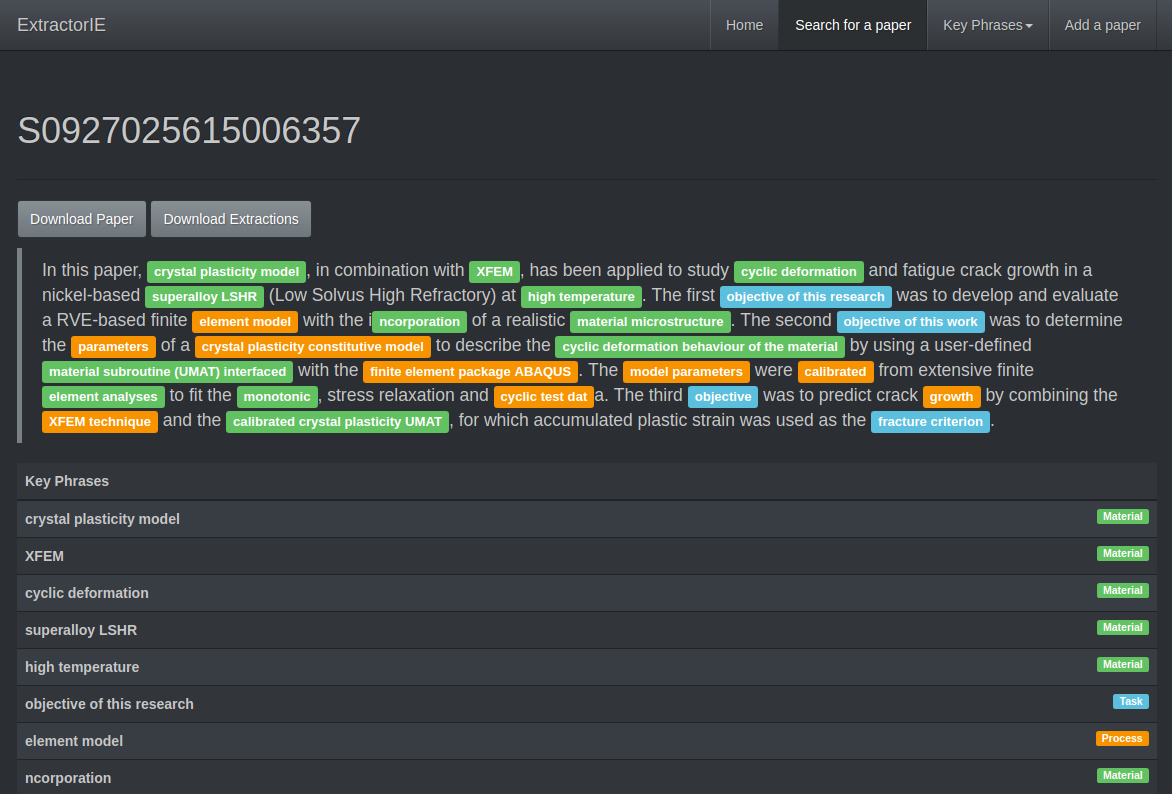
\includegraphics[width=12cm]{img/extractorie-view.png} \\
	\caption[An example view page of the website]{The view page, with a paper's content being shown.}
	\label{figure:extractorieview}
\end{figure}

Using Bootstrap allowed for neat and uniform layouts, with full support for both mobile and desktop browsers. This mean text scaled correctly so should always be easy to read, along with dynamic resizing of important elements such as tables. Furthermore, Bootstrap has label styling, which was utilised to help highlight the classifications of key words. Throughout the project, Bootstraps' \textit{info} (blue), \textit{warning} (orange) and \textit{success} (green) colours were used for marking tasks, processes and materials respectively. Keeping this consistent styling helps make sure the user can quickly understand new information presented, without having to relearn what graphical components mean. The strongest use of the labels is on the view page, where the text (on a dark background) is greeted with bold highlighted areas where key phrases are, making the key information stand out. This can be seen in figure \ref{figure:extractorieview}.

\subsection*{Data Visualisations}
To present the proposed data visualisations, JavaScript solutions were searched for. This would allow the visualisations to be rendered in browser, which reduces the bandwidth required by a image, and can be made to scale depending upon the size of the screen (desktop or mobile).

\begin{figure}
	\centering
	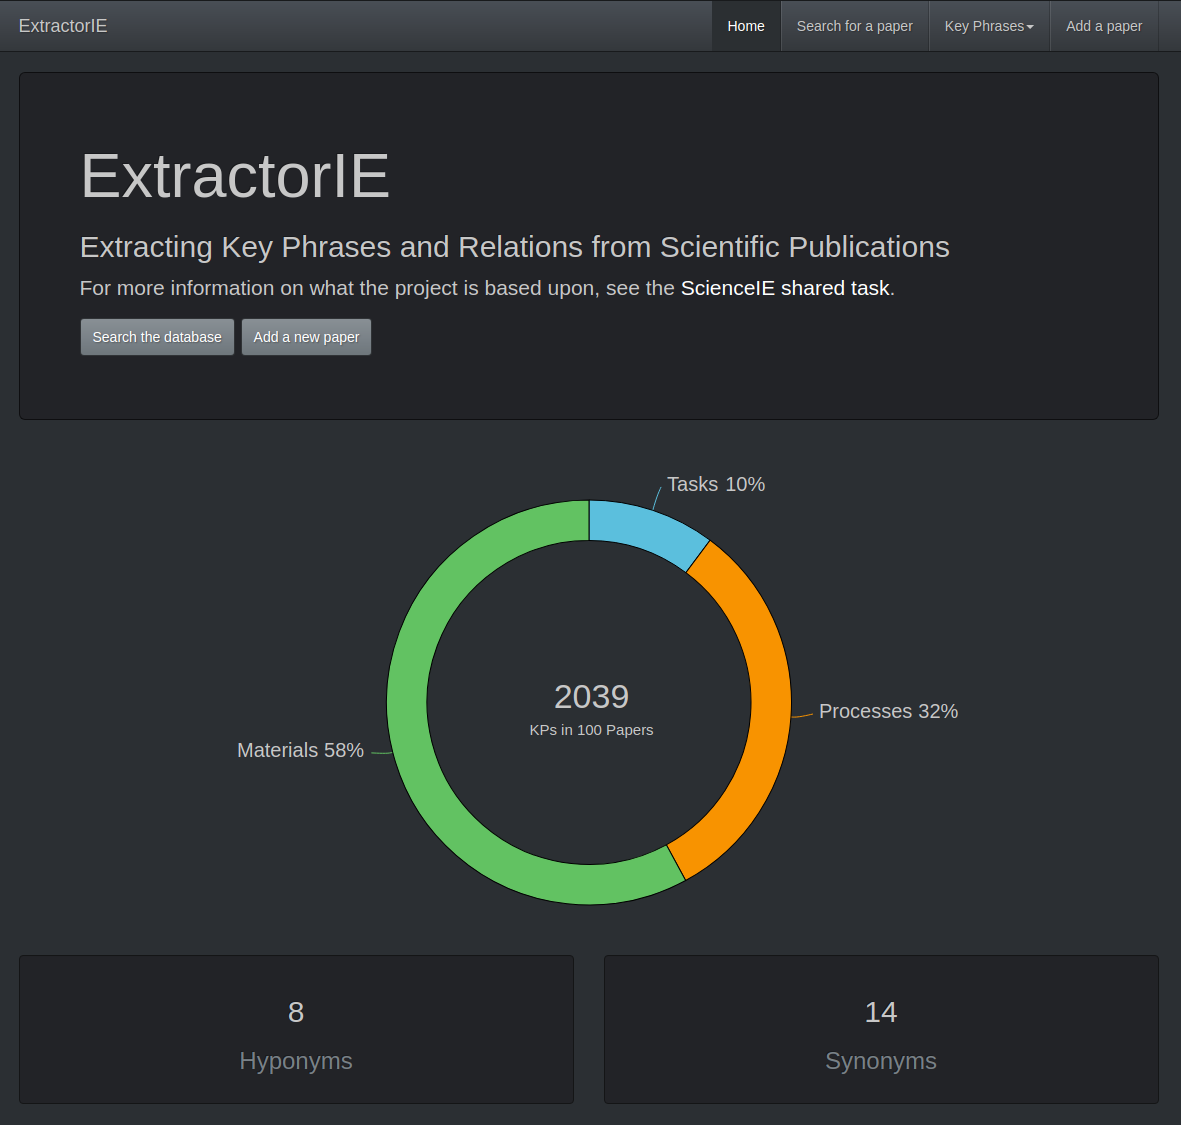
\includegraphics[width=12cm]{img/extractorie-home.png} \\
	\caption[The home page of the website]{The home page of the website, with the pie chart visualisation.}
	\label{figure:extractoriehome}
\end{figure}

For the pie chart, it was found the D3.js could be used to create interactive visualisations, and a third party source allowed simple creation of a donut chart\footnote{\href{https://d3js.org/}{https://d3js.org/} is the base technology, with \href{http://d3pie.org/}{http://d3pie.org/} being used to create a custom donut chart with ease.}. The donut chart generated was set to have overall information in the centre of the chart (including key phrase count and paper count), with the segments being labelled as to the class they represent and the percentage of key phrases they represent. Furthermore, the centre of the chart was made clickable, taking the user to the word cloud page, and the segments were made clickable, taking the user to a list of all key phrases under the given classification. This all results in a lightweight chart that quickly shows some key pieces of information about the contained data, in an interactive way which engages the user. There is even a loading animation included which shows the segments growing, to draw user attention to the visualisation. This is an important chart as it is part of the home page of the system, so being fast to load and show off the information clearly is critical. The segments are also the correct colours to match the rest of the website. The final results can be seen in figure \ref{figure:extractoriehome}.

\begin{figure}
	\centering
	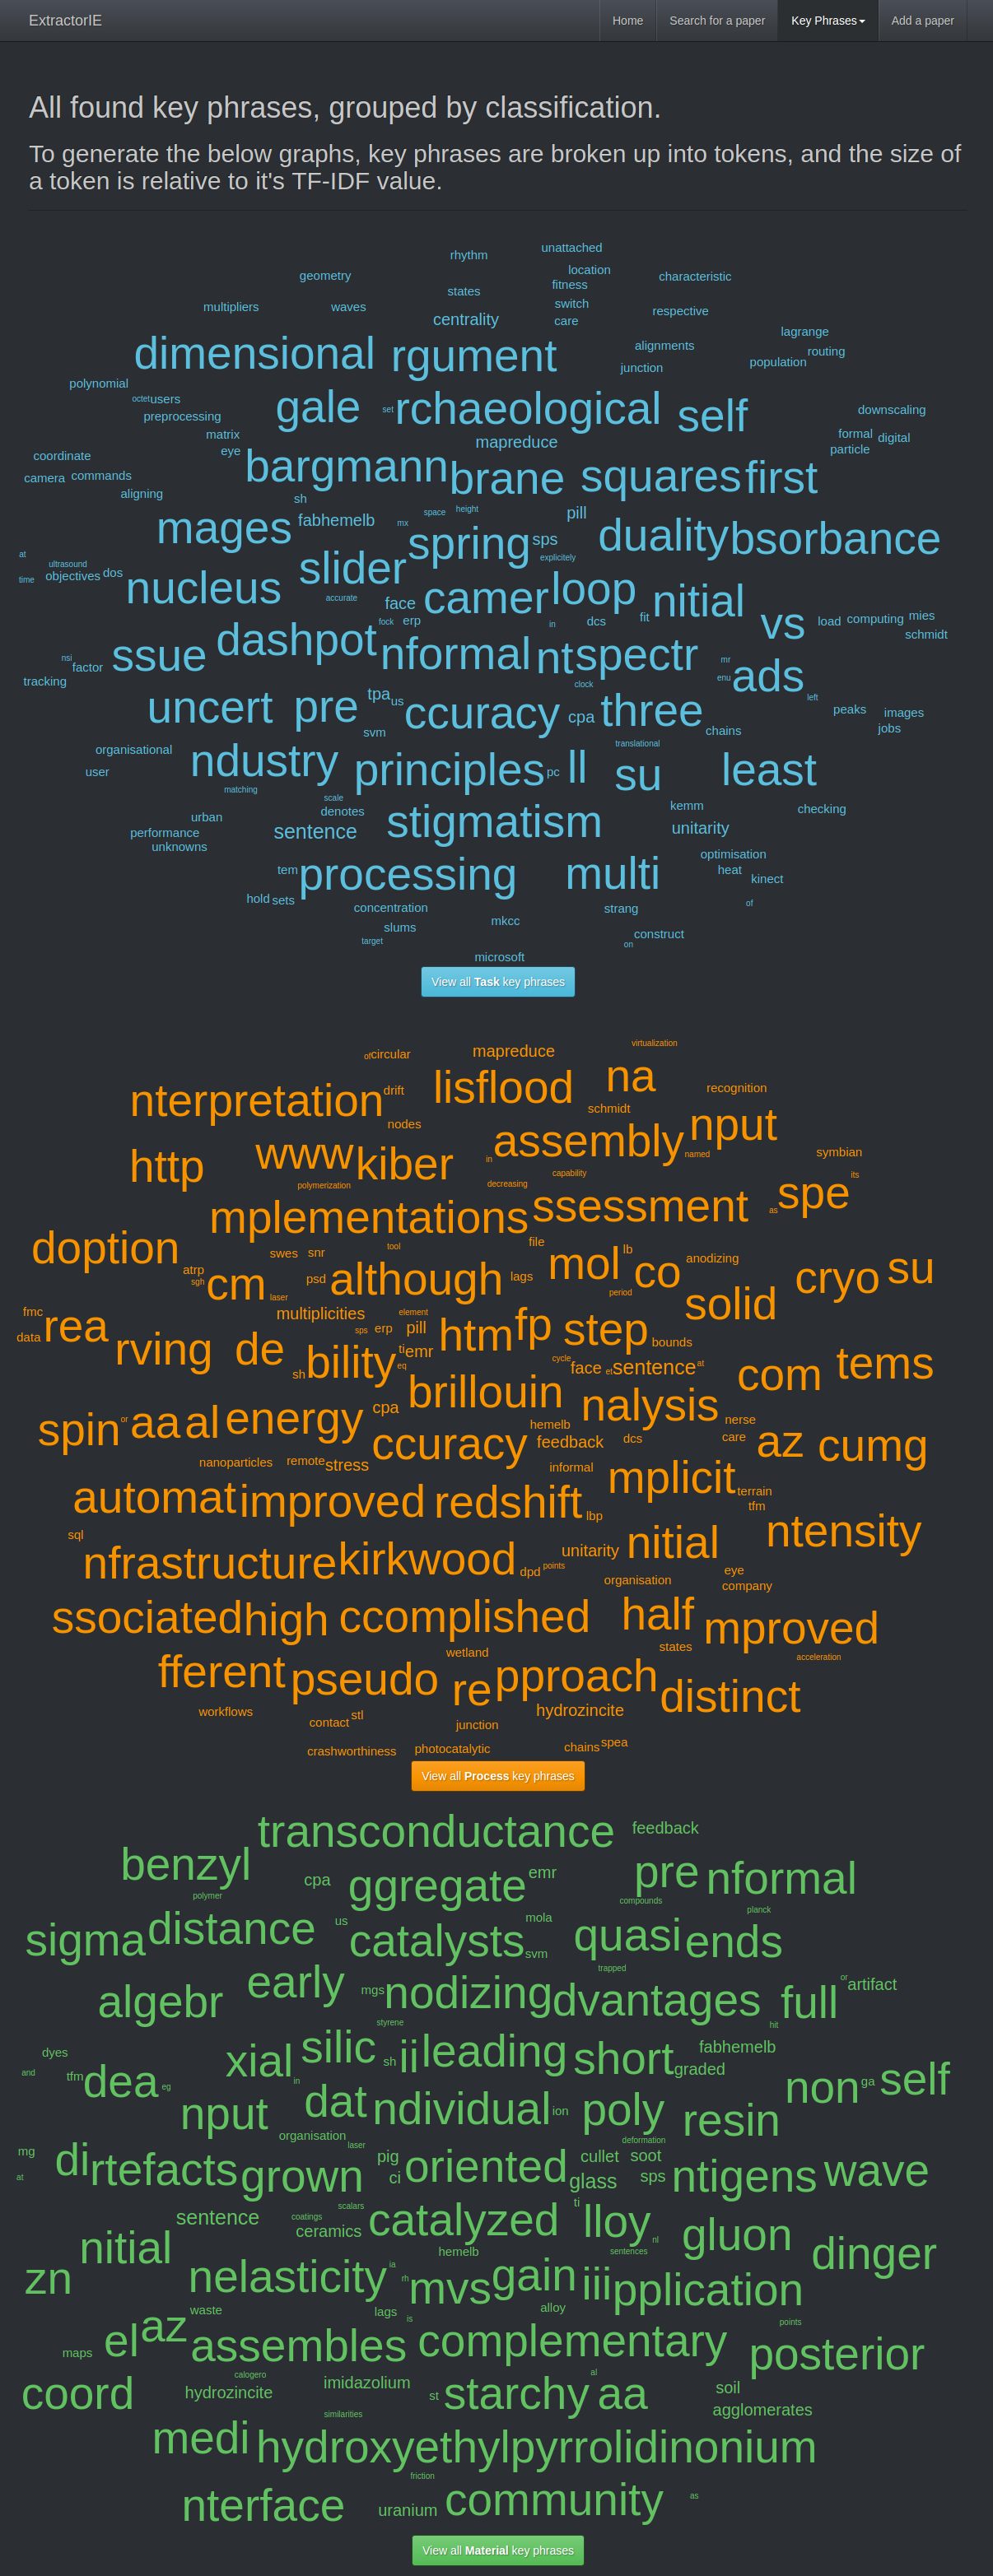
\includegraphics[width=9cm]{img/extractorie-kp.png} \\
	\caption[The home page of the website]{The page containing the three word clouds, one for each classification. The value used to determine a words size is the words TF-IDF.}
	\label{figure:extractoriecloud}
\end{figure}

To achieve the word cloud visualisation, D3.js was again investigated, but a simpler solution using jQuery as a base was found. A third party library called jQCloud\footnote{\href{http://mistic100.github.io/jQCloud/}{http://mistic100.github.io/jQCloud/}} was found which supported the input of a JavaScript array of objects, where each object has a string field and a value field which is what determines the size of the string field when drawn. This is why the \texttt{KPView} controller has a method which returns JSON, as this called be called and its response piped into the jQCloud constructor function. AJAX was used to call the \texttt{KPView} controller three times, once for each classification, and passed the result, when it arrived, to the JQCloud drawing function which draws the cloud of the page. Links under each cloud to a full list of all key phrases with that classification are also provided. The final product can be seen in figure \ref{figure:extractoriecloud}.

\subsection*{The Search Page}

\begin{figure}
	\centering
	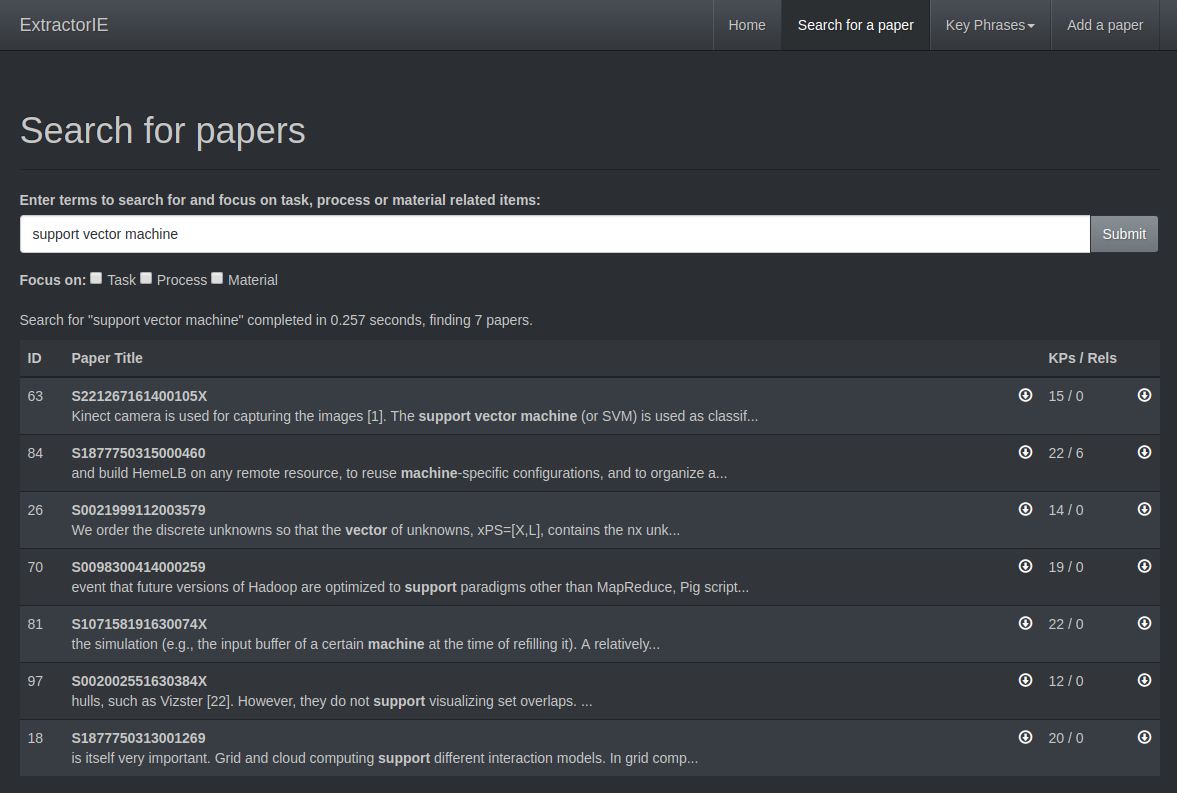
\includegraphics[width=12cm]{img/extractorie-search-supportvectormachine.png} \\
	\caption[An example search of the website]{The search page of the website, with "support vector machine" queried.}
	\label{figure:extractoriesearch}
\end{figure}

The search page consists of a few simple inputs, seen at the top of figure \ref{figure:extractoriesearch}. It allows for any string to be input, along with a set of check boxes for the user to clearly indicate a focus.

Upon searching, the back end is called which returns a list of \texttt{SearchResult} objects, contained in a \texttt{SearchResultAndDetails} which holds some extra information. The extra information given includes the number of search results and the time the search took (inspired by the example websites' feedback to the user) which are both displayed just below the search bar (shown on the screen shot). The search results themselves are shown in a table. This has a main column which contains the title of the paper and a snippet. This snippet contains the piece of text in the document (plus or minus a few words) containing the related query term (with the specific words being in bold, again inspired by the example websites). The key phrase and relation counts for the papers listed are also shown on the right. Next to the title of the paper, is a \textit{quick download} button which is a way for the user to skip to the document rather than load the websites \texttt{/view} page for that paper. A similar idea is presented for relations (downloading the annotation data) on the far right next to the counts.

While not shown in the screen shot, the list is capped at 10 items. After 10 items have been drawn (if there are more than 10 items to draw), a final row is appended with the text "Show X more", where X is the number of results hidden. Clicking on this row reveals the remainder of the results. This is so the user is not overloaded with a large amount of text and information as soon as the search returns. 

\section{Testing}
Testing consists of checking the functionality of the website, as well as evaluating the useful or effectiveness of the implemented requirements.

\subsection*{Strict Testing}
There are a set of strict ways the websites functionality can be tested. A test plan was constructed, which covered the following aspects:
\begin{itemize}
	\item All links on all pages take the user to the correct destination, without an error.
	\item Typing in a random URL returns the correct error page with a 404 message.
	\item The two input fields accept all English letter and numbers without throwing an error (due to a badly formed string).
	\item If the targeted result of the input fields (finding papers or adding a record to the database fails), a reasonable error message is displayed.
	\item When more than 10 papers are displayed at once on the search page, all those after 10 are hidden behind the \textit{view more} button.
	\item Downloading a \texttt{.txt} or \texttt{.ann} file always completes without error.
	\item With respect to the browser window shape/size at load time, both visualisations display readable text and the text does not leave the screen.
\end{itemize}

The website was brought up to a standard where all of the above were complied with, aside from when downloading \texttt{.ann} on macOS with Safari, as it automatically appends \texttt{.txt} to the end of it. Unfortunately, this could not be avoided as it is was diagnosed as a default feature of Safari on macOS.

In terms of browser compatibility, the above tests were carried out on the following browsers on various platforms: Microsoft Edge (Windows 10, Android), Google Chrome (Windows 10, Android), Firefox (Windows 10, Android) and Safari (macOS). 

\subsection*{Requirement Evaluation}
In terms of the simple display requirement, this was achieved well. Taking several pieces of information from the example search engines, the list of papers available (as a result of a search) are displayed in a uniform way, with the title and relevant snippets shown. There are links to an internal page for the paper, as well as quick download links. These are very useful when trying to make a collection of papers or key pieces of information, without having to load individual page to view each paper. This is where one downside presents itself, in that each paper's page has to be loaded individually: unfortunately due to the method used to make the links clickable, middle-click cannot be used, so papers can not be opened in a new tab or window for later viewing. This would be a useful feature to include, as it would allow a user to make a backlog of papers they are interested in reading while they continue to browse.

Furthermore, with regards to the paper display pages, the overall conveying of information is very clear, with boldly highlighted key phrases, and a listing for even more clarity is placed below. Unfortunately, hyponyms and synonyms were not annotated, and while it would have a positive point to have made them available, given the NLP system being used a library to generate this information struggles to make many or high quality relations, not showing this information in a graphical way has no major impact on the user. All of this information is still available in the annotation download. The solution implemented was appropriate for the length of papers being shown, however, this would not be suitable if using full papers instead. If full publications were being displayed, the generated web page would be extremely long, and the design of this may need to be reconsidered.

In terms of search, the overall outcome was positive but not definitive. If the user completed a query, and then changed the focus, given suitable selection of papers were originally found, the order would change. This was verified as being a suitable change by individually checking the key phrases of the papers listed and ensuring the correct classifications of key phrases (as searched for) were being promoted. However, it is hard to definitively call this a success, as to properly test this ideally many hundreds or thousands papers would have been in the database and processed. This would allow for a greater selection of examples to search for and experiment with, and when focussing the effect of different weightings of key phrases could have been investigated further. The use of asynchronous execution when conducting the search was a sensible addition, as it significantly decreased the search time for most queries, however, the time still needed to be displayed to the user as system feedback as some searches could still take some time. 

Furthermore, the search results page was built with the size of the data set in mind. With a maximum of 100 results that could be returned, simply hiding those past the initially readable limit was reasonable for this project. However, that cause significantly problems in terms of data transfer and browser stability if the document pool was scaled up to thousands of records, which could overload the user and the browser. Ideally, pagination should be implemented to cope with many more documents, allowing hte user to progress through small selections at a time.

% TODO example of query showing search working??

% TODO why does time need to be shown to the user

The functionality to support adding papers to the system for automatic processing, and that processing being conducted, was a great success. While the feature didn't support web resources (which would not have been suitable as generally they are quite long), it effectively used the NLP system from earlier in the project to build the database with all of the predicted information. The pending documents would automatically be retrieved from the database and the changes committed, including the extra synonyms found from the sanitisation additions from subtask A's SVM. The only issue that kept occurring, especially when completing processing for subtask C, was that the program kept running out of allocated memory. This caused an exception to be throw, and left a paper at a time in an \textit{error} state, while the error was not caused by the paper itself but the system encountering a problem. Furthermore, in the case of subtask C, if it ran out of memory while processing one paper, it would like do the same for the follow up papers in that instance. Therefore, the code was added to catch memory exceptions, and not run the final subtask again if it crashed once. Otherwise, the system performed as expected, and the data could immediately be viewed on the website. A small addition made to the paper view page was a progress bar being shown if a paper was still undergoing processing (which filled up as it progressed through each stage of processing).

\begin{figure}
	\centering
	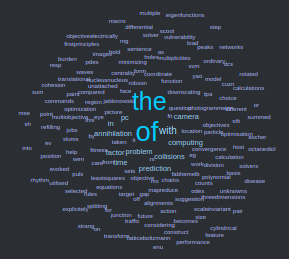
\includegraphics{img/cloud-bad.png} \\
	\caption[The Word Clouds with Word Occurance As The Size Metric]{An example word cloud with word occurrence being used to determine the words size. This did not work as effectively as using TF-IDF.}
	\label{figure:extractoriecloud-bad}
\end{figure}

Finally, the two visualisations created were effective. The first was placed on the home page of the website, which quickly gave new users an indication of the information contained. This linked through to the second page, giving the website a good flow. The cursor would also change to a \textit{hand} (for selecting items) when it was moved across the visualisation, helping to indicate it could be pressed. The word cloud visualisations were less useful, although still interesting to see. As each key phrase was tokenized, no selection of words shown made any grammatical sense, which detracted from the concept of giving users ideas of the key pieces of information selected in this system, as few complete piece of information was shown as one string. Furthermore, due to the removal of odd symbols, some strings occasionally looked odd, for example some were missing letters, or were the combination of two words (where they would have been separated by some symbol, but that symbol was removed). The two values for the words proposed were both examined, and (as predicted) TF-IDF functioned better. The TF-IDF value is used in figure \ref{figure:extractoriecloud}, which clearly has lots of large words at the centre of each cloud which are unusual words, with more common words being smaller and surrounding these big words. Basing the size of words on their occurrence count merely made most of the words small, with very common and unuseful words like "the" and "of" very large at the centre, shown in the example in figure \ref{figure:extractoriecloud-bad}.

\section{Conclusion}
Overall, the proof of concept demonstrating a use for the ScienceIE data has produced a well developed website, including two visualisations and a reasonably competent search engine. It clearly displays information, and can generate more with the use of the NLP system as a library. Some compromises in design were made, such as to display the whole text of a document on the view page and to not include pagination in search (which would be a problem if longer and more publications were added to the system), but overall the system performs well. From a usability point of view, the Bootstrap styling supports most browsers and platforms, and adequate feedback is given to users where needed (such as confirmation messages when a document is submitted for processing and the time of searches).
